% dSIBP package paper.
% Compile: pdflatex paper && bibtex paper && pdflatex paper && pdflatex paper
\documentclass[11pt,a4paper]{article}
\usepackage{jheppub}
\usepackage[T1]{fontenc}
\usepackage{bm}

\title{\bf dSIBP: a package for generating IBP seeds for QFT in de Sitter spacetime}

\author{a}
\affiliation{a}

\abstract{
\texttt{dSIBP} is a \textsc{Mathematica} package. It generates canonical
integration-by-parts (IBP) seed relations for the Feynman integrals of quantum field theory in
de Sitter spacetime. The input is a Feynman graph with massive and massless propagators of the four
Schwinger--Keldysh types. The package builds the corresponding integral family with structured
integer labels. It applies the equation-of-motion and endpoint-state normalizations of the
loop-integral formalism of de Sitter field theory. It then emits canonical seed equations in which
every discrete label has been reduced to a finite basis. The seeds are exported through a
backend-neutral linear-system format to the external reducers Kira and Rational Tracer. The reduced
master integrals can be differentiated to obtain differential equations in a single command. The
package covers arbitrary loop order and arbitrary topologies. It supports the parity-split IBP
system specific to de Sitter time integrals, and it provides a parallel tree-level track that
produces differential equations without any loop momentum. We describe the notation, the public
interface, and worked examples ranging from the sunrise graph to a mixed loop-plus-tree family with
eighty-one master integrals.
}

\begin{document}
% jheppub typesets the table of contents itself as part of \maketitle, so none is written here.
\maketitle

\section{Introduction}

Correlation functions of quantum fields in de Sitter spacetime are computed in the in-in
(Schwinger--Keldysh) formalism. In this formalism the time integrals run over two branches,
and internal lines come in massive and massless variants that connect equal or opposite branches
\cite{Chen:2017ryl}. In momentum space every graph reduces to scalar integrals over the conformal
times $\tau_v<0$ of its vertices. The integrand is a product of plane waves $e^{\mp i E_v \tau_v}$
and of Hankel functions. These time integrals differ from the loop integrals of flat-space field
theory. Under IBP reduction \cite{Chetyrkin:1981qh,Kotikov:1990kg,Laporta:2000dsw,Henn:2013pwa} they
produce linear relations among integrals whose discrete labels count both propagator powers and the
powers of the Hankel functions at the endpoints of each propagator. The dimension of this label
space grows rapidly with the loop order. The reduction therefore becomes the dominant computational
cost of any high-loop calculation in de Sitter space.

The systematic IBP structure of de Sitter time integrals was developed in
refs.~\cite{Chen:2023iix,Chen:2024glu,Chen:2026dqp}. Single-vertex and two-vertex families admit
closed-form IBP relations. Multivariate hypergeometric techniques solve the two-vertex massive
families \cite{Chen:2024glu}. The loop-momentum formalism with a parity-split IBP system covers
general graphs \cite{Chen:2026dqp}. In this formalism the IBP identities take a canonical form in
which every discrete label is confined to a small finite set. The full linear system of a graph is
therefore fixed once the topology, the propagator types and a few kinematic declarations are given.
Writing these canonical seeds by hand is laborious and error-prone already at one loop. Each
propagator carries three structured labels. Massive lines obey second-order equations of motion.
Massless same-branch propagators must be treated as a quotient over endpoint states.

\texttt{dSIBP} is a \textsc{Mathematica} package that automates this step. The user declares a
Feynman graph by its vertices, by the four Schwinger--Keldysh types of its internal lines, and by
its external momenta. The package then performs the following tasks.

\begin{itemize}
\item It validates the kinematic declarations, namely the loop momenta, the no-loop external
magnitudes and their dynamical rules. It reports whether the user lists are complete or
over-complete.
\item It constructs the integral family $J$ with structured labels for propagator powers, endpoint
states and user-defined irreducible scalar products (ISPs).
\item It generates canonical IBP seed equations from the time generators at all active vertices and
from the $L(L+K)$ loop-momentum generators. The massive endpoint states are restricted to the
proven representative set $\{0,1\}$.
\item It sweeps the continuous labels over a user-specified envelope and assembles a sealed,
backend-neutral linear system.
\item It exports the system to Kira \cite{Maierhofer:2017gsa,Klappert:2020nbg} or Rational Tracer
\cite{Magerya:2022hvj} for the actual reduction, and it imports the results back.
\item It differentiates the reduced master integrals with respect to the independent kinematic
variables. This yields differential equations, optionally in $d\log$ form. Euler scaling identities
provide an independent check of the result.
\end{itemize}

The package generates and serializes IBP relations, but it never runs a reduction itself. The
reduction is delegated to external programs. This separation keeps the package independent of any
particular reduction engine. A complementary tree-level track provides seed relations for
single- and multi-vertex time-only families. These seeds can be reduced internally to differential
equations and $d\log$ forms without any loop momentum. The track also interfaces with the package
MadStree \cite{MadStree:inpreparation}, which evaluates tree-level cosmological correlators
numerically. Related structures for cosmological loop integrands appear in the kinematic-flow
program \cite{Fan:2024iek,Hang:2024xas,Baumann:2024mvm}.

All formulas used by the package are derived in
refs.~\cite{Chen:2023iix,Chen:2024glu,Chen:2026dqp}; the package adds no new derivation. The purpose
of this paper is therefore to state the notation in a complete and self-contained form
(section~\ref{sec:notation}), and to describe the public interface
(sections~\ref{sec:using} and~\ref{sec:examples}). Every symbol that appears in the output of the
package is traced back to its definition. The interface described below is that of the current
public release.

\noindent\textbf{Statement on AI use.}
The notation, the functionality and the interfaces of \texttt{dSIBP} were designed by the author.
The author supervised a number of different agent programs and large language models that
implemented the code and the documentation. The author also designed the validation tasks that
establish the reliability of the package. All of these tasks are cross-validations of computed
results against independent data. They cover the IBP relations, the differential equations and the
scaling identities as follows.

\begin{itemize}
\item \emph{Massive two-vertex family.} The general IBP seeds and the differential equations are
checked against the analytic results of ref.~\cite{Chen:2024glu}. The family has five normalized
masters. The three $5\times5$ differential-equation matrices agree entry by entry, $25/25$ exact in
each matrix. The vertex basis and the ordering of the masters follow ref.~\cite{Chen:2023iix}.
This task validates the IBP relations and the differential equations.
\item \emph{Massive three-vertex tree family.} The formulas were first derived independently by an
agent, which generalized an earlier hand-written two-vertex implementation. They were checked
against ref.~\cite{Chen:2026dqp} and only then compared with the output of the package. This task
validates the tree-level IBP relations and the tree-level differential equations.
\item \emph{One-loop bubble, full pipeline.} The IBP system is reduced by an external Kira run,
which closes with no unreduced target and returns nineteen masters. The two $19\times19$
differential-equation matrices keep both derivative variables symbolic. At the recorded exact point
they reproduce the matrices of ref.~\cite{Chen:2026dqp} entry by entry, $361/361$ for each of the
three variable conventions. The scaling identities hold on the reduced basis: $33/33$ source-level
identities and $19/19$ active-basis checks pass symbolically. This task validates the IBP relations,
the differential equations and the scaling identities.
\item \emph{Mixed bubble-plus-tree family, full pipeline.} The family has eighty-one master
integrals. The external Kira reduction closes with no unreduced target. The six $81\times81$
differential-equation matrices are free of residual symbols. All $81/81$ source-level Euler scaling
and IBP identities vanish exactly. These identities are independent of the numerical reduction. The
reduction itself carries a scaling certificate at a recorded exact point. This task
validates the IBP relations, the differential equations and the scaling identities.
\item \emph{General formulas against naive sampling.} The package substitutes the derived general
formulas instead of solving IBP systems again. Its output was compared with reductions of naively
sampled raw IBP seeds of the same families. The IBP relations and the differential equations agree.
This task validates the IBP relations and the differential equations.
\item \emph{Tree-level differential equations against MadStree.} The direct $d\log$ route and the
naive IBP route of the package give the same result. In addition, for a mixed three-vertex tree
family with fifteen masters, the parameter derivatives of \texttt{dSIBP} were transported into
MadStree \cite{MadStree:inpreparation} for the five variables $k_1,k_2,k_3,\texttt{sE}1,\texttt{sE}2$.
All seventy-five derivatives closed, and the five $15\times15$ differential-equation matrices agree
entry by entry with the direct $d\log$ formula route of MadStree. This task validates the
tree-level differential equations.
\end{itemize}

\noindent The package is available at \url{https://github.com/J7C/dSIBP-Packages}.

\section{Notation and conventions}
\label{sec:notation}

\subsection{Schwinger--Keldysh Feynman rules}
\label{sec:skrules}

A de Sitter Feynman graph in the in-in formalism consists of vertices $v$ with conformal time
$\tau_v<0$ and Schwinger--Keldysh branch signs $\sigma_v=\pm$. Each vertex with external energy
$E_v$ carries the phase factor
\begin{equation}
e^{-i \sigma_v E_v \tau_v}\,,
\label{eq:vertexPhase}
\end{equation}
and the time integrations run over the full interval $\tau_v\in(-\infty,0)$. An internal line $e$
that connects the vertices $u$ and $v$ is one of four types. It is massive or massless, and it is
full (same branch, $\sigma_u=\sigma_v$) or cross (opposite branch, $\sigma_u=-\sigma_v$). The four
propagator types have distinct Heaviside structures and different kernels. The massive full and
cross propagators differ by a factor $i$, and the two massless cross propagators likewise differ by
a factor $i$. The massless full propagator is the sum of its two ordered halves. In our figures a
circle denotes a vertex, and its fill colour encodes the branch sign: black is $\sigma_v=+$, white
is $\sigma_v=-$, and gray leaves the sign general. The conformal time $\tau_v$ is written below the
vertex and the vertex energy beside it. External legs end in small open squares. The energy $E_v$
of a vertex is the sum of the magnitudes of all external momenta routed into $v$, plus any vertex
energy parameter $z_v$. Figure~\ref{fig:skrules} shows these rules for the bubble input of the
package. Its two vertices are drawn in gray because their branch signs are general. Vertex~1
carries the external momenta $k_{1,1},\dots,k_{1,n_1}$ and vertex~2 carries
$k_{2,1},\dots,k_{2,n_2}$. The internal momenta are $q$ and $q-k$.

\begin{figure}[t]
\centering
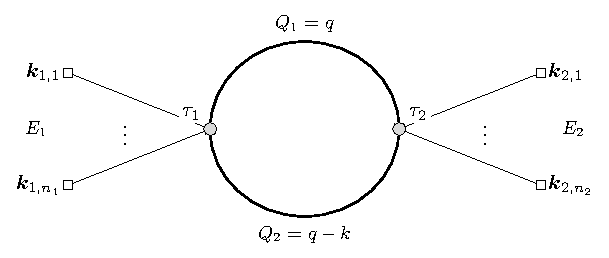
\includegraphics{figures/fig_skrules.pdf}
\caption{Feynman rules of a de Sitter bubble with general branch signs, drawn as gray vertices.
The vertex energies $E_1,E_2$ and the conformal times $\tau_1,\tau_2$ are written at the vertices.
The external legs end in open squares and carry the momenta $k_{1,1},\dots,k_{1,n_1}$ and
$k_{2,1},\dots,k_{2,n_2}$. The two internal lines carry the loop momenta $q$ and $q-k$.}
\label{fig:skrules}
\end{figure}

The package distinguishes the four internal-line types as
$\langle$\texttt{massive, massless}$\rangle\times\langle$\texttt{full, cross}$\rangle$.
Figure~\ref{fig:linetypes} shows the resulting graphical conventions. Every cyclic line of the
graph becomes a propagator of the integral family. Non-cyclic lines attached to the loop skeleton
are \emph{fixed lines}. They carry only a magnitude power and no loop-momentum denominator. Massive
lines whose endpoints become coincident under a contact operation may be \emph{shrunk}. Shrunk
lines survive only through a structured prefactor of the sector.

\begin{figure}[t]
\centering
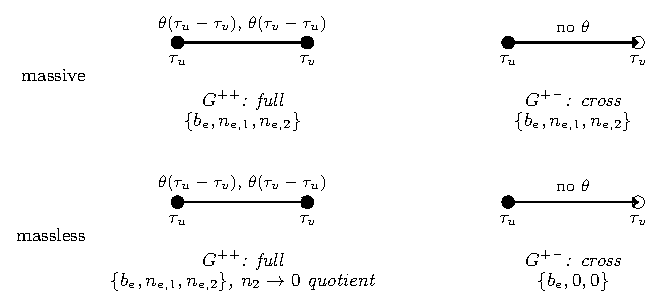
\includegraphics{figures/fig_linetypes.pdf}
\caption{The four internal-line types and their label packs. The fill colour of a vertex encodes
its branch sign: black is $+$ and white is $-$. The conjugate assignments $--$ and $-+$ give the
same two line types. Massive and massless full lines carry $\{b_e,n_{e,1},n_{e,2}\}$, with the
massive endpoint states restricted to $\{0,1\}$. Cross lines carry $\{b_e,0,0\}$. Massless full
lines are the quotient of the two ordered endpoint states, with $F_{01}=-F_{10}$ and
$F_{11}=-F_{00}$.}
\label{fig:linetypes}
\end{figure}

\subsection{The integral family}
\label{sec:family}

For a sector $s$, that is, a subset of propagators retained as denominators, a generic member of
the integral family is a time-ordered integral over the vertex times,
\begin{equation}
\begin{split}
J[s,\{a_v\},\{B_e,n_{e,1},n_{e,2}\},\{\rho_r\}]
={}&\int_{-\infty}^{0}\prod_v d\tau_v\;
\prod_v (-\tau_v)^{a_v+a0_v}\, e^{-i\sigma_v E_v \tau_v}\\
&\times\prod_{e\in s} \mathcal{G}_e(\tau_u,\tau_v)^{B_e}\;
\prod_{e} H_e^{n_{e,1}}\,\bar H_e^{n_{e,2}}\;
\prod_r \rho_r^{\,i_r}\,.
\end{split}
\label{eq:family}
\end{equation}
Here $e=(u,v)$ runs over the lines of the sector, $\mathcal{G}_e$ is the propagator of the line $e$,
and $H_e,\bar H_e$ are the Hankel-function blocks attached to the two endpoints of a massive line.
In the package the family is written in the three-slot schema
\begin{verbatim}
J[sectorKey_String, linePacks_List, ispList_List]
\end{verbatim}
The first slot identifies the sector by the retained propagators. The second slot holds one pack
per line, in the root line order.

\begin{itemize}
\item A cyclic full line contributes $\{b_e,n_{e,1},n_{e,2}\}$: the propagator power $b_e$ and the
Hankel powers at the two endpoints.
\item A cyclic massless cross line contributes $\{b_e,0,0\}$.
\item A fixed line contributes $\{\texttt{"F"},n_{e,1},n_{e,2}\}$: no denominator power, only the
magnitude powers of the line.
\item A shrunk line contributes $\{b_{S,e}\}$, the magnitude power kept by the sector prefactor.
\end{itemize}

\noindent The third slot lists the ISPs with their integer indices $i_r$.

The zero points of the labels are fixed by the package and cannot be changed by the user. For the
$h$-preset dynamics the vertex time powers have $a0_v=2\nu_{\mathrm{ref}}$, and the massive
propagator powers have $b0_e=-2\nu_e$. The \emph{actual} powers that enter the integrand are
therefore $A_v=a_v+a0_v$ and $B_e=b_e+b0_e$, while the package-level labels $a_v,b_e,n_{e,i}$ run
over small non-negative integers. These conventions follow
refs.~\cite{Chen:2024glu,Chen:2026dqp}. They make the IBP shifts uniform: the generators shift the
package-level labels by $\pm1$ and never touch the zero points.

\paragraph{Massive endpoint states and equations of motion.}
A massive line $e$ with mass parameter $\nu_e$ and the $h$-preset $P_h(x)=(2\nu_e+1)/x$,
$Q_h(x)=1$ has Hankel blocks at each endpoint that span a two-dimensional space. The space is
indexed by the state $n_{e,i}$. The second-order equation of motion gives, at $n_{e,i}=2$, the exact
relation
\begin{equation}
\begin{split}
J\big[\cdots,n_{e,i}=2,\cdots\big]
={}&-J\big[\cdots,n_{e,i}=0,\cdots\big]\\
&-(2\nu_e+1)\,J\big[\cdots,n_{e,i}=1,\,a_r\to a_r-1,\,b_e\to b_e+1,\cdots\big],
\end{split}
\label{eq:eom}
\end{equation}
so every massive endpoint state reduces to the representative set $\{0,1\}$. The package applies
this reduction by construction: the generated seeds contain only $n_{e,i}\in\{0,1\}$.

\paragraph{Massless quotient.}
A massless full line does not distinguish its two endpoints. The package fixes an ordered state
$(n_{e,1},n_{e,2})$ per line and works with the quotient
\begin{equation}
F_{01}=-F_{10},\qquad F_{11}=-F_{00},
\label{eq:masslessQuotient}
\end{equation}
so the public family keeps a single bit per massless full line, taken from the representatives
$F_{00}$ and $F_{10}$. This is an exact algebraic identification, not a sampling prescription.

\paragraph{Shrink rules.}
A massive line may be shrunk only in the \texttt{massiveFull} type and only when
$n_{e,1}+n_{e,2}=1$. The shrink multiplies the sector by the coefficient
$-\chi_e(-1)^{n_{e,r}}C_e$, where $\chi_e=\pm1$ is fixed by the two vertex types and
$C_e=\tfrac{4i}{\pi}e^{\pi\,\mathrm{Im}\,\nu_e}$. A massless full line shrinks with a $\mp2$ delta
term and a $+2$ term, without a Wronskian prefactor and without label shifts. If all lines meeting
at a vertex shrink simultaneously, the odd-subset contact terms
\begin{equation}
\sum_{\substack{\emptyset\neq S\subseteq B\\ |S|\ \mathrm{odd}}} 2^{\,1-|S|}
\prod_{e\in S} D_e \prod_{e\in S} J_e
\label{eq:contact}
\end{equation}
are generated. Shrunk lines never reappear as denominators. Their magnitude powers live in the
structured sector prefactor.

\subsection{Kinematics}
\label{sec:kinematics}

The structural loop number $L$ is the first Betti number of the internal undirected multigraph.
Let $E$ count the internal edges: parallel edges are counted once per line, and each self-loop
contributes one edge. External legs do not contribute to $E$. Let $V$ count the vertices and $C$
the connected components. Then
\begin{equation}
L=E-V+C\,.
\label{eq:loopnumber}
\end{equation}
Together with $K$ independent
loop-related external momenta, the loop number fixes the number of scalar products,
\begin{equation}
N_{\mathrm{sp}}=\frac{L(L+1)}{2}+LK\,.
\label{eq:nsp}
\end{equation}
The user
declares two separate lists. The first list, \texttt{loopExternalMomenta} $\{k_1,\dots,k_K\}$,
defines the loop coordinates $\texttt{ss}ij=\sqrt{\mathrm{sp}[k_i,k_j]}$ of the loop Gram matrix.
The second list, \texttt{independentExternalMomenta}, defines the no-loop magnitudes
$|\texttt{kE}i|$ that appear in vertex energies and fixed-line masses. These magnitudes are
parameterized by $\texttt{sE}i$. Only
magnitudes are coordinates. The package never outputs $\mathrm{sp}[k_{Ei},k_{Ej}]$, and it never
eliminates intermediate magnitudes by a cosine rule. Magnitudes that depend on the declared ones
are stored as explicit bindings. They still contribute to vertex phases through the chain rule.

User-defined ISPs are declared as \texttt{name/expr/range} associations, for example
\begin{verbatim}
<|"name" -> rho1, "expr" -> sp[q1, k], "range" -> {0, 1}|>,
\end{verbatim}
and they must form an invertible coordinate system on the space of scalar products together with
the propagator squares. The definition zero point of an ISP is fixed at $0$: positive powers are
numerator powers, and a negative power means an extra denominator. Kinematic rules of the form
$\mathrm{sp}[k_i,k_j]\to$ dynamical variables are validated by the two-stage interface
\texttt{DSKinematics}/\texttt{DSInit}. The interface reports exact, over-complete or under-complete
states. Only the exact state opens derivative generation.

\subsection{Parity structure}
\label{sec:parity}

The characteristic discrete invariant of de Sitter IBP is the parity of the sum of the line labels.
For every cyclic line $e$ the quantity
\begin{equation}
p_e \;=\; b_e+n_{e,1}+n_{e,2} \pmod 2
\label{eq:parity}
\end{equation}
is invariant under all loop and time generators acting on a full massive line. It is preserved by
the $h/H$ shrink of massive lines. For massless full lines it flips by construction: the contact
operation maps $b_e+n_{e,1}+n_{e,2}\to b_e+1$, so the massless parity of a shrunken sector is offset
by one. Cross lines carry no parity constraint. Every generator preserves the parity vector
$(p_e)_e$. The IBP system of a family therefore splits into independent parity blocks. For families
with user-provided \texttt{parityConstraints} the package restricts the seeds to the requested
block, for example $b_{[1]}+n_{[1,1]}+n_{[1,2]}\equiv0$. This reproduces the parity-split IBP system
of ref.~\cite{Chen:2026dqp}. ISP indices receive no parity filter.

\subsection{Dynamical rules and massive function systems}
\label{sec:dynamics}

Every massive line is assigned a second-order function system
$f_e''+P_e(x)\,f_e'+Q_e(x)\,f_e=0$. The default \texttt{"h"} preset uses $P_h=(2\nu_e+1)/x$ and
$Q_h=1$. The package also accepts bare Hankel functions $H$ and general user systems $(P,Q,T,W)$.
Let $T_e$ be the transport matrix of the fundamental system and $W_e$ its Wronskian. The package
tracks the combination $W_T=\det(T)\,W$ through all shrinks. The theta-coincidence and Wronskian
shrink terms used by the time-IBP generators are derived from it. Ordinary derivatives of dynamical
quantities never generate theta shrinks and never invoke $W_T$. The user chooses the convention
once at initialization. The IBP generators, the derivative operators and the tree-level track all
read the same compiled function system.

\subsection{Tree-level and time-only families}
\label{sec:timeonly}

For graphs without cycles the package exposes a \texttt{timeOnly} family with the unique public
representation
\begin{verbatim}
J[sectorKey_String, timeShifts_List, stateBits_List]
\end{verbatim}
Here \texttt{sectorKey} records, per root line, whether the line is full (1) or shrunk (0). The list
\texttt{timeShifts} gives the time powers $a_v$ of the active vertices. The list \texttt{stateBits}
gives one bit per massive endpoint or massless quotient state, in the frozen root-line order. There
are no momentum generators, no propagator powers and no ISPs. Fixed-line magnitude powers remain in
the structured sector prefactor and still enter derivative generation. The massive-only time-only
families are fully certified. Families that contain massless full lines are returned as
\texttt{PendingRederivation}. The reason recorded with them is
\texttt{masslessQuotientFormulaNotCertified}. The public
interface does not bypass this gate.

\section{Using the package}
\label{sec:using}

\subsection{Initialization}

A case is a named topology declaration. Initialization runs a structural audit of the loop number,
the vertex and line registry and the external-momentum routing. It then runs the kinematic audit of
section~\ref{sec:kinematics}. The result is a context that every later command consumes:
\begin{verbatim}
context = DSInit[case, KinematicRules -> custom];
\end{verbatim}
The optional two-stage interface \texttt{DSKinematics[case]} first returns a proposal with the
default rules and a selection template. The user can then inspect the kinematic coordinates
$\texttt{ss}ij,\texttt{sE}i$, the momentum-routing audit and the capability flags before committing.
Under-complete declarations abort the initialization. Over-complete ones allow symbolic seed
generation but disable derivatives and the inner-form rewriting. In the over-complete case common
loop shifts are quotiented out through an affine basis \texttt{effectiveLoopExternalMomenta}.

\subsection{Seeds and the IBP envelope}
\label{sec:seeds}

\texttt{DSSeeds[context]} returns the canonical seed templates of the family. Every actual sector
receives all active time generators and all $L(L+K)$ loop-momentum generators. The massive endpoint
states are pre-reduced by the equation of motion \eqref{eq:eom}. Massless full lines run over the
two quotient representatives. The discrete $n$ labels are eliminated, and the analytic seeds keep
general continuous labels $a_v,b_e,b_{S,e}$ and general ISP indices. Each template is hash-sealed.
Templates that the equation of motion and the canonicalization reduce to the identity $0=0$ are
retained and audited rather than dropped.

The continuous labels are swept by \texttt{DSGenerateIBP}. The unified form
\begin{verbatim}
ibpData = DSGenerateIBP[allSeeds, {-1, 1}];
\end{verbatim}
requires that every root continuous index lies in the closed integer interval $[-1,1]$ \emph{after}
all shifts of the generated relations. The package inverts the per-index shift sets and derives the
narrower seed ranges automatically. The per-index form
\begin{verbatim}
ibpData = DSGenerateIBP[allSeeds,
   {a[v1], -1, 1}, {a[v2], 0, 1},
   {b[e1], 0, 2}, {b[e2], -1, 1}];
\end{verbatim}
must cover all root continuous indices exactly. ISP lower bounds are combined with the user target
by taking the larger lower bound, so the package never extends a range on its own in order to cover
numerator terms. The output is a sealed contract with status \texttt{"generated"}, a template-set
hash, an integrity audit and the capability flags \texttt{sealedQ}, \texttt{completeSystemQ} and
\texttt{subsetQ}. Only sealed complete systems may proceed to a formal reduction.

\subsection{Linear systems and external reduction}
\label{sec:linear}

\texttt{DSLinear[ibpData, context]} converts the sealed seeds into a backend-neutral association
\texttt{linearData}. Its fields are the equation list \texttt{linearEquations}, the master-integral
ordering \texttt{integralList}, the pivot rules \texttt{integralRules}, the sector metadata
\texttt{sectorMetadataList} and the readiness reports. The order of \texttt{integralList} fixes the
master-integral ordering. The command \texttt{DSReorderIntegrals} re-indexes it if
the user prefers a different order. The two-stage Kira plan is built purely in memory:
\begin{verbatim}
prePlan   = DSKiraPlan[linearData, <|"stage" -> "preReduction", ...|>];
preExport = DSKiraExport[prePlan];
(* ... external Kira run identifies the master integrals ... *)
userMIData = DSUserMI[linearData, userExpressions, <|
   "names" -> activeNames, "activeIndices" -> activeIndices,
   "derivativeVariables" -> {ss11, P0}, "scalingDegrees" -> degrees|>];
formalPlan   = DSKiraPlan[linearWithUserMI, <|"stage" -> "formal", ...|>];
formalExport = DSKiraExport[formalPlan];
(* ... external Kira run reduces to the user basis ... *)
importedData = DSKiraImport[formalWorkspace];
\end{verbatim}
The pre-reduction stage freezes the candidate targets and lets the external reducer discover the
masters. The command \texttt{DSUserMI} then attaches the user basis. It checks the global and the
active rank, and it stores reversible pivot rules. The formal stage constructs the analytic
derivative closure of the active basis \emph{before} any export. It refuses to write if internal
helper symbols survive. Export manifests carry the SHA-256 identity of every artifact, and
\texttt{DSKiraImport} re-verifies the contents instead of trusting version strings. The serializer
maps momenta to the imaginary axis $k\to-I\,ik$ expected by Kira. The same \texttt{linearData}
feeds the Rational Tracer \cite{Magerya:2022hvj} pipeline through the equation-system interface.

\subsection{Differential equations and checks}
\label{sec:de}

After the reduction, \texttt{DSDE} differentiates the master integrals with respect to the
independent variables. Loop-Gram coordinates are handled through external-vector derivative
decompositions. No-loop magnitudes are handled through line-local radial derivatives, including
their dependent bindings. Vertex energies enter as scalar parameters. Explicit coefficients are
differentiated directly, while bare integrals are shifted and canonicalized. The result is reduced
back to the active basis. For the pure massive bubble the resulting equations are in $d\log$ form.
At the recorded exact point they reproduce the matrices of ref.~\cite{Chen:2026dqp} entry by entry.

Every integral of the family is a homogeneous function of the dimensionful variables. Let
$x_1,\dots,x_m$ denote these variables, that is, the loop coordinates $\texttt{ss}ij$, the no-loop
magnitudes $\texttt{sE}i$ and the mass scales. Each master integral $I_k$ then satisfies the Euler
relation
\begin{equation}
\sum_{a=1}^{m} x_a\,\frac{\partial I_k}{\partial x_a} \;=\; d_k\, I_k\,,
\label{eq:euler}
\end{equation}
where $d_k$ is the constant scaling degree of $I_k$. In matrix form, with
$\partial I/\partial x_a=A_a(x)\,I$, the identity \eqref{eq:euler} becomes
\begin{equation}
\sum_{a=1}^{m} x_a\, A_a(x) \;=\; \Delta\,,\qquad
\Delta=\mathrm{diag}(d_1,\dots,d_N)\,.
\label{eq:eulerMatrix}
\end{equation}
The command \texttt{DSScaleCheck} verifies \eqref{eq:eulerMatrix} symbolically on the reduced basis.
It also checks the source-level time and loop-momentum IBP identities before the reduction. Because
$\Delta$ is constant and diagonal, \eqref{eq:eulerMatrix} is a strong self-consistency test of the
whole chain from seeds to differential equations. The tree-level track exposes
\texttt{DSTreeDLogDE} for direct $d\log$ differential equations.

At the atomic level the package also exposes the generators themselves:
\begin{verbatim}
dtau[i, expr, context]     (* time generator at vertex i *)
dqq[i, j, expr, context]   (* d/dq_i . q_j *)
dqk[i, j, expr, context]   (* d/dq_i . k_j *)
ds[expr, var, context]     (* full variable derivative *)
\end{verbatim}
together with the form rewriters \texttt{rep2innerform}, \texttt{rep2outform} and
\texttt{rep2Integrand}. The last command expands a $J$ into its explicit integrand without
integrating. The short signatures rely on the single registered topology. Explicit contexts should
be used when several topologies are alive.

\subsection{Tree-level track}
\label{sec:tree}

The tree-level functions mirror the loop workflow:
\begin{verbatim}
treeSeeds = DSTreeSeeds[context];
iterative = repIterative[treeSeeds, context];
naiveIBP  = DSTreeNaiveIBP[treeSeeds, context];
naiveDE   = DSTreeNaiveDE[naiveIBP, context];
dlogDE    = DSTreeDLogDE[iterative, context];
\end{verbatim}
The iterative route substitutes the general derived formulas directly. The naive route reduces raw
sampled IBP relations. The two routes must agree, and the package reports the flag
\texttt{deRoutesAgree}. The tree-level differential equations have also been compared with the
package MadStree \cite{MadStree:inpreparation}. MadStree evaluates tree-level cosmological
correlators and builds its own $d\log$ differential equations. For a mixed three-vertex tree family
with fifteen masters, the parameter derivatives
of \texttt{dSIBP} were reduced by MadStree for the five variables
$k_1,k_2,k_3,\texttt{sE}1,\texttt{sE}2$. All seventy-five derivatives closed, and the five
$15\times15$ matrices agree entry by entry with the direct $d\log$ formula route of MadStree.
Figure~\ref{fig:workflow} summarizes the two tracks and their connection to
the external reducers. Appendix~\ref{app:api} lists the public functions with one-line
descriptions.

\begin{figure}[t]
\centering
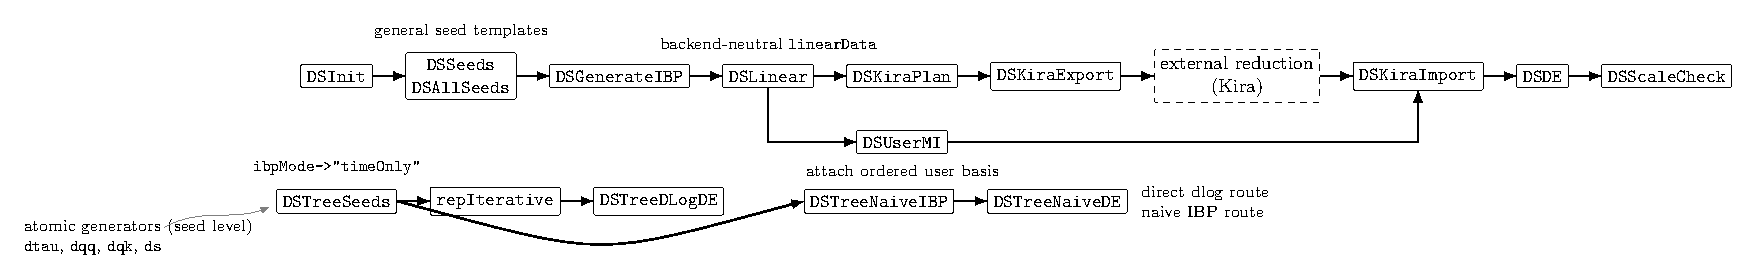
\includegraphics[width=0.98\textwidth]{figures/fig_workflow.pdf}
\caption{The public workflow of \texttt{dSIBP}. Full (loop) families run from \texttt{DSInit}
through the seed, envelope and linear-system stages to the two-stage Kira export and import and to
the differential-equation layer. The command \texttt{DSUserMI} attaches the user basis between the
two reduction stages. Tree-level (\texttt{timeOnly}) families run through \texttt{DSTreeSeeds} and
\texttt{repIterative} to \texttt{DSTreeDLogDE}, with the naive IBP route as an independent
cross-check. The atomic generators \texttt{dtau}, \texttt{dqq}, \texttt{dqk} and \texttt{ds} are
available at every stage.}
\label{fig:workflow}
\end{figure}

\section{Examples}
\label{sec:examples}

The package ships six worked examples. Figure~\ref{fig:examples} shows the four graphs discussed
below. The quoted Kira times are wall-clock times of the external reduction on a single
workstation. The Kira inputs were written by \texttt{DSKiraExport}.

\begin{figure}[t]
\centering
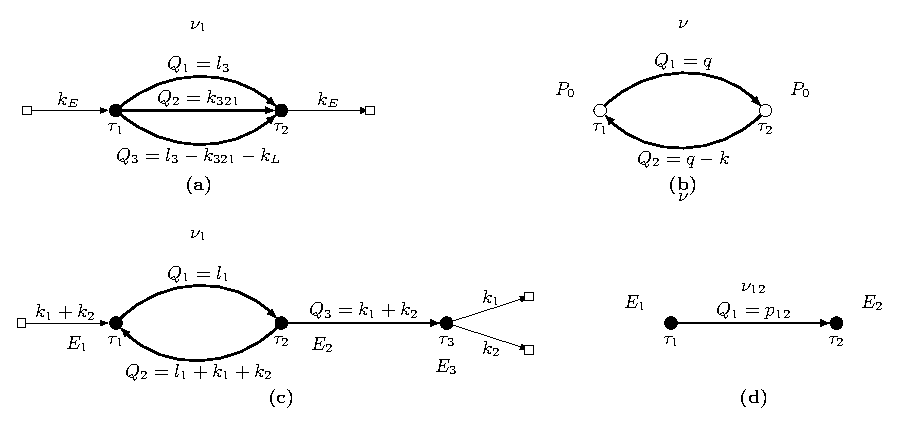
\includegraphics[width=0.97\textwidth]{figures/fig_examples.pdf}
\caption{Example graphs. The fill colour of a vertex encodes its branch sign: black is $+$ and
white is $-$. (a)~The two-loop sunrise of example~03: one massive full line of mass $\nu_1$ and two
massless full lines between two $+$ vertices; both vertices carry the same external-leg energy
$k_E$. (b)~The pure massive bubble of example~04: two massive full lines of the same mass $\nu$
between two $-$ vertices with vertex energy $P_0$; the loop external momentum is $k$. (c)~The
mixed bubble-plus-tree case of example~06: a massive full line of mass $\nu_1$ and a massless full
line form the loop between $v_1$ and $v_2$, and a massless bridge connects $v_2$ and $v_3$; the
external legs carry $k_1+k_2$, $k_1$ and $k_2$. (d)~The two-vertex tree of example~05: a massive
line of mass $\nu_{12}$ whose momentum $p_{12}$ is a no-loop magnitude.}
\label{fig:examples}
\end{figure}

\paragraph{Sunrise (example 03).}
The graph of figure~\ref{fig:examples}a has two vertices and three parallel lines, hence $L=2$.
Line~1 is a massive full line of mass $\nu_1$, and lines~2 and~3 are massless full lines. The loop
momenta are $l_3$ and $k_{321}$, and the single loop external momentum is $k_L$. Thus $K=1$, and
the loop Gram matrix gives the coordinate $\texttt{ss}11=|k_L|$. No no-loop magnitude is declared:
both vertices carry the same external-leg energy $k_E$, which is the second derivative variable.
The top sector receives two time generators and $L(L+K)=6$ loop-momentum generators. Two ISPs are
declared, $\mathrm{sp}[k_{321},l_3]$ and $\mathrm{sp}[l_3-k_{321}-k_L,l_3]$, each with range
$\{0,1\}$. The symmetry that swaps the two massless lines exchanges them, and the package
canonicalizes the two ISPs together with that swap. The example stops after the general stage. It
generates the canonical seeds and the general parameter-derivative operators, and it neither
samples the continuous labels nor runs a reduction, a differential equation or a scaling check. The
seeds are checked by applying \texttt{ds} to the top-sector integral with respect to both
variables.

\paragraph{Pure massive bubble (example 04).}
The bubble of figure~\ref{fig:examples}b has two vertices on the $-$ branch. Its two massive full
lines carry the same mass $\nu$ and the loop momenta $q$ and $q-k$. The loop external momentum $k$
gives the loop coordinate $\texttt{ss}11=|k|$. Both vertex energies are set to the parameter
$P_0$, which is the second derivative variable. This example runs the full closed loop: seeds,
envelope sweep, linear system, two-stage Kira export, external reduction, import, differential
equations and scaling check. The Kira workspace must lie outside the repository, and the package
itself never starts Kira. The linear system is written at a fixed rational probe point for the
dimension and the masses, while the differential equations keep $\texttt{ss}11$ and $P_0$ symbolic.
The reduction closes with no unreduced target and returns nineteen master integrals. The two
$19\times19$ differential-equation matrices in $d\log$ form reproduce those of
ref.~\cite{Chen:2026dqp}: at the recorded exact point each of the three variable conventions agrees
entry by entry, $361/361$. The scaling identities \eqref{eq:eulerMatrix} hold symbolically on the
same basis, with $33/33$ source-level identities and $19/19$ active-basis checks.

\paragraph{Mixed bubble plus tree (example 06).}
The most demanding released case is figure~\ref{fig:examples}c. Lines~1 and~2 form the loop:
line~1 is a massive full line of mass $\nu_1$, and line~2 is a massless full line. Line~3 is a
massless bridge between $v_2$ and $v_3$. It lies outside the loop, so its pack carries no
denominator power. The external legs carry $k_1+k_2$ into $v_1$ and $k_1,k_2$ into $v_3$. The loop
external momentum is $k_1+k_2$, which gives $\texttt{ss}11$. The independent no-loop magnitudes
$k_1,k_2$ give $\texttt{sE}1,\texttt{sE}2$. Both cycle lines are restricted to even parity,
$b_{[e]}+n_{[e,1]}+n_{[e,2]}\equiv0$ for $e=1,2$, while the fixed bridge is excluded from the
parity constraints. The parity-restricted family has eighty-one master integrals, and the generated
system contains 818{,}217 relations. The external Kira reduction takes about 160\,s and closes with
no unreduced target. The package then produces six $81\times81$ differential-equation matrices, one
for each of the variables $\texttt{ss}11,\texttt{sE}1,\texttt{sE}2,E_1,E_2,E_3$, with no residual
symbols. All $81/81$ source-level Euler and IBP identities vanish exactly. The reduction-based
scaling certificate is evaluated at the recorded exact point, because all six scaling variables are
fixed in the formal plan. The example also exercises the parameter redefinition
\texttt{DSRedefineParameters}, a bound-energy coordinate binding $E_0=|k_1|+|k_2|$, and the
over-complete and under-complete kinematic audits.

\paragraph{Two-vertex tree (example 05).}
A massive line of mass $\nu_{12}$ connects two $+$ vertices, figure~\ref{fig:examples}d. There is
no loop momentum. The momentum $p_{12}$ of the line is declared as an independent no-loop magnitude,
so the package builds the coordinate $\texttt{sE}1=|p_{12}|$. The \texttt{timeOnly} family has the
two sector keys \texttt{"1"} and \texttt{"0"}, for the full and the shrunk line. The iterative route
and the naive IBP route give the same $d\log$ differential equations in $E_1,E_2,\texttt{sE}1$, so
\texttt{deRoutesAgree} is \texttt{True}. The same example also declares a one-line massless family.
Its quotient states reduce to $n_{1,1}\to0$, $n_{1,1}\to1$ and $n_{1,2}\to0$ over the sector keys
\texttt{"0"} and \texttt{"1"}. Its formula route returns \texttt{PendingRederivation} with the
reason \texttt{masslessQuotientFormulaNotCertified}, as required by the gate of
section~\ref{sec:timeonly}.

\paragraph{Mixed bubble workflow and bare Hankel system (examples 01, 02).}
Example~01 declares a bubble with one massive and one massless full line between two $+$ vertices.
It runs the unified public entry through the discrete templates, the continuous sweep and the
linear system. It builds the pre-reduction plan in memory without exporting or running Kira.
Example~02 supplies a bare Hankel function system $(P,Q,T,W)$ instead of the \texttt{"h"} preset.
The package compiles it through the same public workflow and generates the seeds of the
corresponding family. Together the two examples cover the initialization, the envelope sweep and
the function-system interface of sections~\ref{sec:using} and~\ref{sec:dynamics}.

\section{Summary and outlook}

\texttt{dSIBP} turns the canonical IBP structure of de Sitter time integrals into a practical
\textsc{Mathematica} tool. From a graph declaration it produces sealed canonical seeds,
backend-neutral linear systems, Kira and Rational-Tracer export manifests with artifact identities,
differential equations and scaling checks. It covers arbitrary topologies that mix massive and
massless propagators of all four Schwinger--Keldysh types. The parity-split structure, the massive
equation-of-motion reduction and the massless quotient are applied by construction, so the user
never handles raw label spaces. Ongoing work concerns the certification of the massless full-line
tree-level formulas, which are currently gated behind \texttt{PendingRederivation}. Further
directions are a deeper integration with hypergeometric solution methods \cite{Chen:2024glu} and
the connection to numerical evaluation pipelines such as MadStree
\cite{MadStree:inpreparation} and to high-precision series-transport solvers \cite{Liu:2022chg}.

\section*{Acknowledgements}

We thank the developers of Kira \cite{Maierhofer:2017gsa,Klappert:2020nbg}, Rational Tracer
\cite{Magerya:2022hvj} and MadStree \cite{MadStree:inpreparation} for making their tools available.

\appendix

\section{Public functions}
\label{app:api}

\renewcommand{\arraystretch}{1.15}
\begin{center}
\begin{tabular}{p{4.3cm}p{9.8cm}}
\hline
\textbf{Function} & \textbf{Description} \\
\hline
\texttt{DSInit} & initialize a case; structural and kinematic audits; returns the context. \\
\texttt{DSKinematics} & two-stage kinematic proposal and validation. \\
\texttt{DSParameterNotation} & inspect the current parameter notation. \\
\texttt{DSRedefineParameters} & replace the dynamical rules; re-audits and rehashes. \\
\texttt{DSSeeds} & canonical seed templates of a family. \\
\texttt{DSAllSeeds} & flattened seed template list. \\
\texttt{DSSeedGroups},\newline\texttt{DSSeedGroupMetadata} & grouping of the templates by sector, class and generator. \\
\texttt{DSMetaSeedRange} & per-group shift metadata for envelope planning. \\
\texttt{DSGenerateIBP} & sweep continuous indices; sealed IBP relations. \\
\texttt{DSLinear} & backend-neutral linear system (\texttt{linearData}). \\
\texttt{DSReorderIntegrals} & re-index the master-integral ordering. \\
\texttt{DSKiraPlan} & in-memory pre-reduction or formal reduction plan. \\
\texttt{DSKiraExport} & write Kira input directories; manifest with SHA-256 identities. \\
\texttt{DSKiraImport} & read back external reduction results with identity checks. \\
\texttt{DSUserMI} & attach a user master-integral basis with rank checks. \\
\texttt{DSDE} & differential equations of the reduced basis. \\
\texttt{DSScaleCheck} & Euler scaling identities of the family. \\
\texttt{DSTreeSeeds} & \texttt{timeOnly} seed templates. \\
\texttt{repIterative} & tree route via the general derived formulas. \\
\texttt{DSTreeNaiveIBP},\newline\texttt{DSTreeNaiveDE} & tree route via raw sampled IBP. \\
\texttt{DSTreeDLogDE} & tree $d\log$ differential equations. \\
\texttt{dtau}, \texttt{dqq}, \texttt{dqk}, \texttt{ds} & atomic generators and the full variable derivative. \\
\texttt{rep2innerform},\newline\texttt{rep2outform} & notation rewriters between user and internal forms. \\
\texttt{rep2Integrand} & expand $J$ into the explicit integrand. \\
\texttt{symmetry} & apply user and gated self-loop symmetry rules. \\
\hline
\end{tabular}
\end{center}

\bibliographystyle{JHEP}
\bibliography{references}

\end{document}
